% ******************************* Thesis Appendix A ****************************
\chapter{Snow characteristics for the Carpathian Region} 

% **************************** Define Graphics Path **************************
\ifpdf
    \graphicspath{{Appendix1/Figs/Raster/}{Appendix1/Figs/PDF/}{Appendix1/Figs/}}
\else
    \graphicspath{{Appendix1/Figs/Vector/}{Appendix1/Figs/}}
\fi

%\section{Static snow maps}

%related to Chapter \ref{cha:stat_unc} and \ref{cha:time_trend}

\section{Interactive snow map}
\label{sec:int_snow_map}

An online, interactive snow map is developed, which can be used to obtain characteristic ground snow load and other structural engineering related snow information for the Carpathian region (Figure \ref{fig:int_snow_map}). The database presented in Section\,\ref{sec:data_under_study} is used for the map.

\begin{figure}[htbp!]
	\centering    
	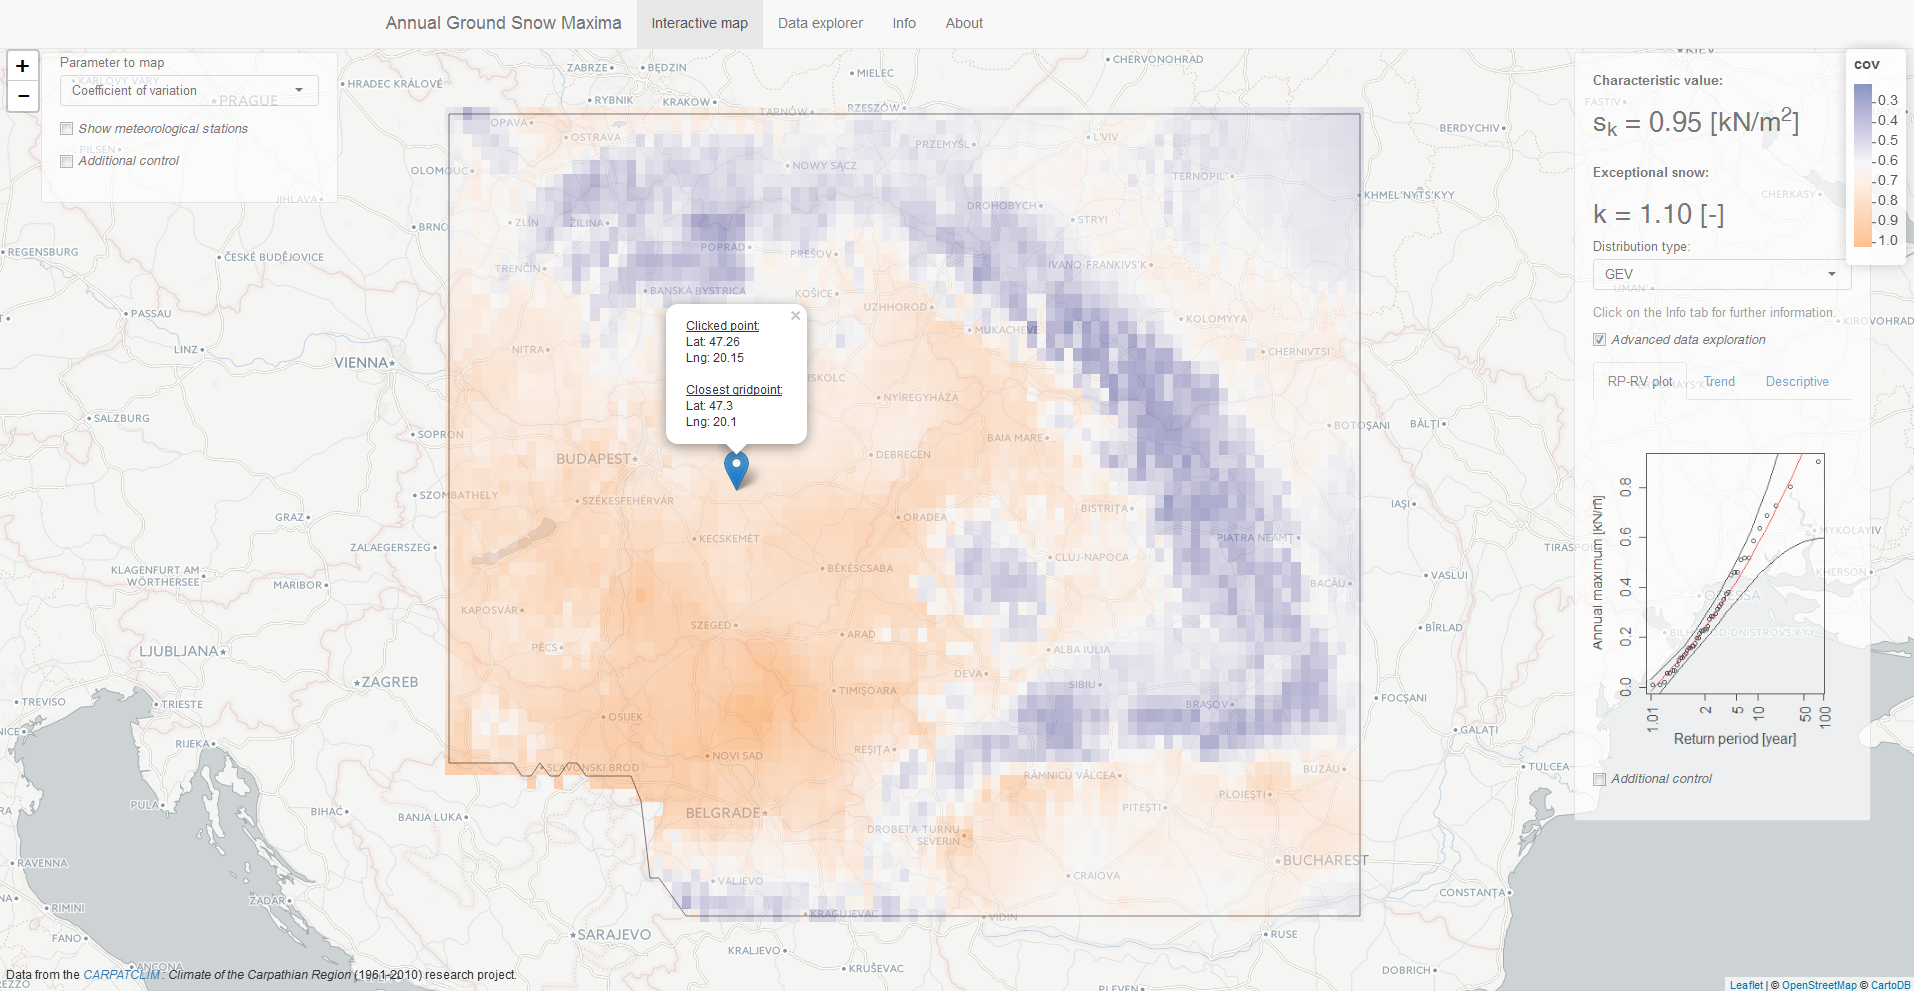
\includegraphics[width=1\textwidth]{online_snow_map_illustration.png}
	\caption{Screenshot of the interactive snow map.}
	\label{fig:int_snow_map}
\end{figure}

\noindent
The source code and an online running instance is available on this page:\\
\url{https://github.com/rozsasarpi/Interactive-snow-map-R}

\medskip
\noindent
The interactive map is motivated by the:
\begin{itemize}
	\item often appreciable change in snow maps, ground snow load, and other snow related measures by crossing national borders;
	\item largely inaccessible previous snow related research even within the seeker's own country, this is the case for Hungary;
	\item principles of open and reproducible research;
	\item the need for later update of snow maps, which is hoped to be eased by the published code;
	\item need for site specific loading conditions;
	\item difficulty of analyzing, exploring large datasets.
\end{itemize}

These motivations are valid for other actions as well, e.g. seismic actions, and the presented approach of publicly shared codes, databases, and interactivity may help in those cases as well. The application is developed in R \citep{R2015} using shiny \citep{shiny2015}, for details see the source code.


\section{Posterior distribution of GEV parameters}
\label{sec:GEV_posterior}

The posterior distributions of annual ground snow maxima parameters are given here to provide prior information to region with similar climatic conditions (Figure~\ref{fig:GEV_posterior}). The posterior distributions are constructed with the following assumptions and considerations:
\begin{itemize}
	%\item Bayesian analysis used to infer the posterior distributions.
	\item Generalized extreme value distribution is used to formulate the likelihood function.
	\item The posterior distribution of shape, scale, and location parameters are provided.
	\item Distributions are given for lowlands and for highlands as well due to their distinct characteristics.
	\item Uniform priors are used for all parameters with practically infinite range.
	\item The observations for each locations are standardized: centering and scaling (Eq.\ref{eq:stand_obs}).
	\item Three locations are used for each groups, these are far apart from each other to ensure independence (Figure~\ref{fig:posterior_locations}). 
\end{itemize}

The standardization of observations makes it possible to aggregate data from different locations. It is done the following way:
\begin{equation}
\label{eq:stand_obs}
 	{x_{s,i}} = \frac{{{x_i} - m}}{s}
\end{equation}
where:

\begin{tabular}{ll}
	$x_{s,i}$ & $i$th standardized observation; \\
	$x_i$ & $i$th observation; \\
	$m$ & sample mean; \\
	$s$ & corrected sample standard deviation, Eq.\ref{eq:std}.
\end{tabular} \medskip

\begin{equation}
\label{eq:std}
 	s = \sqrt {\frac{1}{{1 - n}} \cdot \sum\nolimits_{i = 1}^n {{{\left( {{x_i} - m} \right)}^2}} } 
\end{equation}
where $n$ is the sample size.

From these parameters the non-standardized parameters or other snow characteristics can be readily obtained with their posterior distributions as well. It requires further analysis to decide which locations can be considered independent in respect of ground snow maxima. The three-three locations are assumed to be independent due to their distance. If more independent locations can be added then the posterior distributions could be greatly improved.

\begin{figure}[htbp!]
	\centering    
	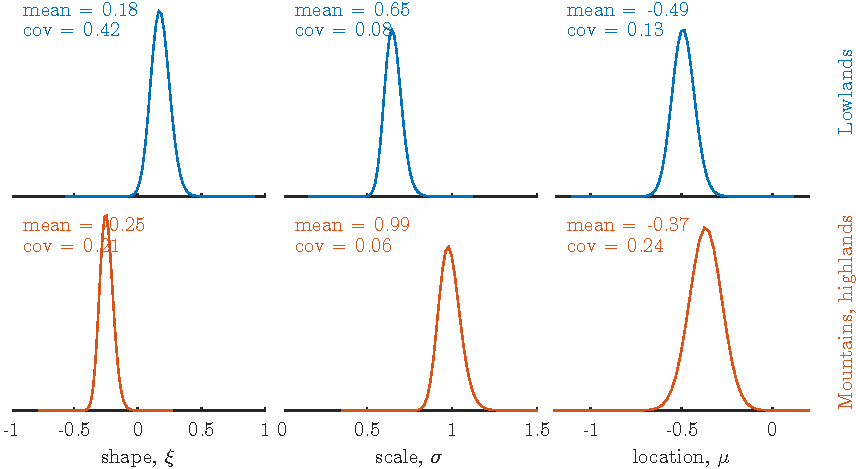
\includegraphics[width=1\textwidth]{GEV_posterior.pdf}
	\caption{Posterior distributions of GEV parameters for the lowlands, and mountains and highlands. Corresponding to standardized observations.}
	\label{fig:GEV_posterior}
\end{figure}

\begin{figure}[htbp!]
	\centering    
	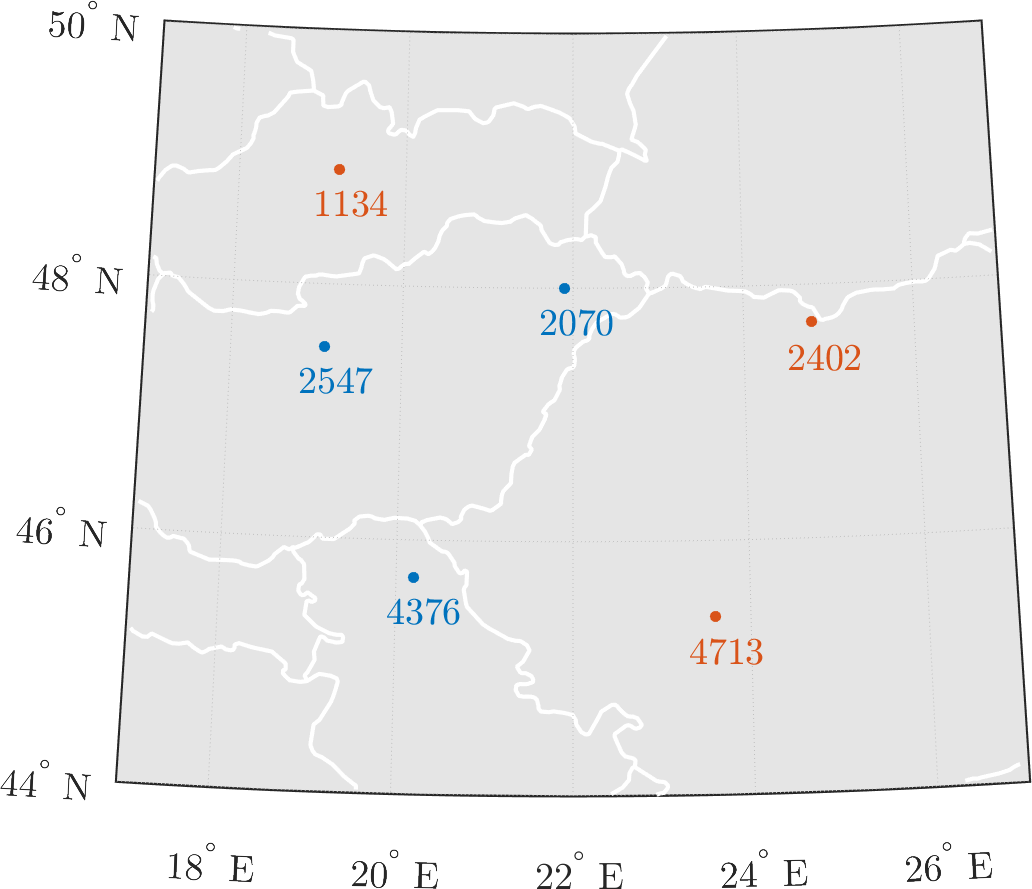
\includegraphics[width=0.7\textwidth]{posterior_locations.png}
	\caption{Position of the selected locations for lowlands (blue), and for mountains and highlands (orange). The numbers are related to the CarpatClim database.}
	\label{fig:posterior_locations}
\end{figure}


%!!!!!!!!!!!!!!!!!!!!!!!!!!!!!!!!!!!!!!!!!!!!!!!!!!!!
\mynote{Mirek: it would useful if it could be indicated in the introduction or somewhere that map will be considered during the next revision of EN1-1-3. Show the practical impact of the work!}
%!!!!!!!!!!!!!!!!!!!!!!!!!!!!!!!!!!!!!!!!!!!!!!!!!!!!

